\documentclass[sigconf]{acmart}

\AtBeginDocument{%
  \providecommand\BibTeX{{%
    Bib\TeX}}}

\setcopyright{none}
\settopmatter{printacmref=false}
\renewcommand\footnotetextcopyrightpermission[1]{}

\usepackage{booktabs}
\usepackage{placeins}
\usepackage{tikz}

\usetikzlibrary{arrows.meta,positioning}

\newcommand{\system}{\textsc{BriskSnapShot}}
\setlength{\textfloatsep}{8pt}
\setlength{\floatsep}{7pt}
\setlength{\abovecaptionskip}{3pt}
\setlength{\belowcaptionskip}{2pt}

\begin{document}

\title{\system{}: A Live Demo of Join-Backed Semantic Windows for Streaming AI Pipelines}

\author{Anonymous Author(s)}
\acmConference[ICPP '26]{The 55th International Conference on Parallel Processing}{September 28--October 1, 2026}{Singapore}
\acmYear{2026}
\copyrightyear{2026}

\begin{abstract}
Streaming AI applications need to keep vector state fresh while exposing that state in a form that downstream services can inspect and act on. \system{} is a live demonstration of a unified semantic-window system built from the SAGE orchestration codebase and the SageFlow vector-stream runtime~\cite{sage_icml2026,sage_repo,sageflow_repo}. The demo follows public vulnerability-intelligence reports as they are normalized, embedded, joined inside a bounded semantic window, and surfaced as snapshot, routing, and escalation contracts. Unlike a static retrieval demo, \system{} lets the audience see how new events change the active window, which vector joins support a cluster, and what compact evidence is handed to an LLM-facing application. A 24-event walkthrough remains small enough for live narration, while expanded 240-event and 2,400-event replays show that the same contract path continues to emit useful evidence under larger streams.
\end{abstract}

\ccsdesc[500]{Computer systems organization~Parallel architectures}
\ccsdesc[500]{Information systems~Stream management}
\ccsdesc[300]{Computing methodologies~Artificial intelligence}

\keywords{stream processing, vector search, AI middleware, semantic windows, demonstration}

\maketitle

\section{Introduction}

Large-model applications increasingly run as long-lived dataflows rather than as isolated prompt calls. A vulnerability assistant receives new advisories while an investigation is still open; a retrieval pipeline refreshes its vector neighborhood between two user questions; an on-call agent must decide whether a new report belongs to a known incident or deserves escalation. In these settings, the model-facing component should not receive an opaque vector index or a free-form prompt dump. It needs bounded, inspectable evidence: which records are retained, which records matched, which sources support the cluster, and which action the system recommends.

Stream processors provide scalable dataflow execution~\cite{akidau2015dataflow,carbone2015apache}, while vector indexes provide efficient approximate search~\cite{jegou2011product,johnson2019billion,malkov2020efficient}. Retrieval-augmented systems further show how language models benefit from external evidence~\cite{lewis2020rag,guu2020realm}. What is still awkward in many prototypes is the boundary between streaming state and AI orchestration. Semantic state is often rebuilt outside the component that observes the stream, so a demo can show an answer but not the live runtime evidence that made the answer possible.

\system{} demonstrates a narrower and more observable boundary. The system owns the active semantic window, runs vector joins as events arrive, and exports only compact contracts to the application layer. A contract is not another prompt; it is a structured object with cluster identity, supporting neighbors, source coverage, novelty, route, priority, and action fields. The demo is built around the question an audience naturally asks during a live system demonstration: when the next event arrives, what changes, why did it change, and what can the upper pipeline safely do with the change?

The paper keeps the original demo narrative but makes three pieces explicit. First, it describes the system architecture as a single integrated prototype rather than two adjacent components. Second, it expands the live demonstration path so that the UI, presenter script, and pipeline stages have clear roles. Third, it adds prepared evidence beyond the 24-event walkthrough, including scale replays and parameter variants that show the capability of the system without turning the paper into a full benchmark paper.

\section{System Overview}

\begin{figure}[t]
  \centering
  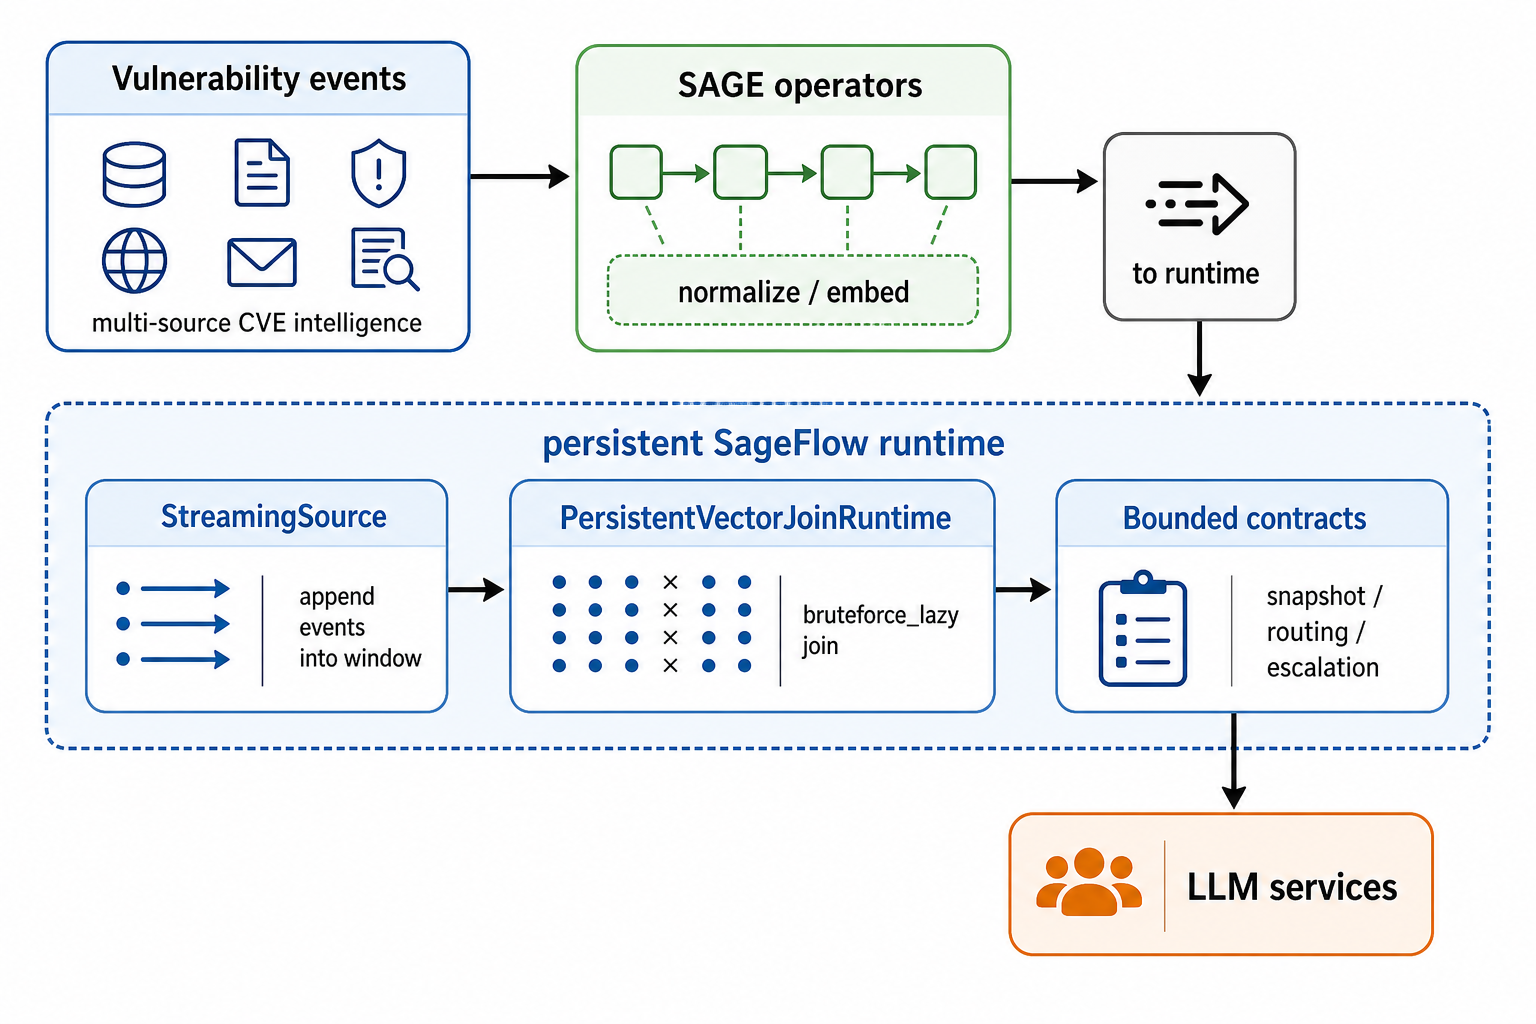
\includegraphics[width=\columnwidth]{figures/brisk_architecture.png}
  \caption{\system{} architecture. Events are normalized and embedded, a persistent vector runtime owns the semantic window and join pairs, and the application layer receives bounded contracts.}
  \Description{Architecture diagram showing vulnerability events entering a normalization and embedding layer, flowing into a vector runtime with a windowed join, and returning bounded contracts to application services.}
  \label{fig:overview}
\end{figure}

Figure~\ref{fig:overview} shows the implemented path. \system{} takes heterogeneous vulnerability reports from multiple sources, maps each report into a deterministic embedding for reproducible demos, appends the record into a bounded semantic window, and drains join pairs produced by the persistent runtime. The output is then folded into application-level contracts. This organization is intentionally close to the way the live demo is presented: the audience first sees an event enter the pipeline, then sees the runtime evidence that connects it to prior records, and finally sees the contract that an application can consume.

\subsection{Design Goals}

The first design goal is \emph{observable freshness}. A static retrieval index can demonstrate relevance, but it hides whether the context is current. \system{} keeps the current window visible: retained records, emitted pairs, active clusters, and newest evidence are all displayed as runtime state rather than as post-hoc explanation text.

The second goal is \emph{bounded handoff}. Model-facing services should not receive an unbounded list of nearest neighbors. The system exports a small set of fields that can be logged, routed, or summarized: cluster identity, source coverage, supporting neighbor identifiers, novelty, route, priority, and action. This turns the semantic window into an application interface rather than a private runtime detail.

The third goal is \emph{demo reproducibility}. Live demos are convincing when they are interactive, but papers also need evidence that the observed behavior is not a hand-picked screen. The same replay driver used for the UI can run deterministic expanded streams, threshold variants, and window-size variants. The prepared figure in Section~\ref{sec:evidence} is generated from those replay artifacts.

\subsection{Runtime Boundary}

\begin{table}[t]
  \centering
  \caption{Runtime boundary exposed by the demo.}
  \label{tab:boundary}
  \begin{tabular}{@{}p{0.28\columnwidth}p{0.58\columnwidth}@{}}
    \toprule
    Component & Demo-visible role \\
    \midrule
    Ingestion layer & Source replay, deterministic embedding, event metadata \\
    Window manager & Bounded retention, reset/cleanup, snapshot export \\
    Join runtime & Left-right append, vector comparison, pair emission \\
    Contract layer & Snapshot, owner route, escalation signal \\
    UI and evidence & Live controls, replay trace, scale summaries \\
    \bottomrule
  \end{tabular}
\end{table}

Table~\ref{tab:boundary} summarizes the system boundary. The ingestion layer gives the runtime comparable vectors and stable identifiers. The window manager owns which events are still active and which events have left the current view. The join runtime is the only component that creates semantic match pairs. The contract layer interprets those pairs for an application: a dense multi-source cluster becomes an incident snapshot, a cluster with a clear owner becomes a routing contract, and a high-severity novel event becomes an escalation contract.

Cluster construction uses connected components over returned join pairs. Clusters are sorted by size and average severity before export, which makes the display stable enough for a presenter to narrate. The default incident rule requires at least three events, average severity above 0.70, and at least two source classes. The emerging-risk rule fires when a high-severity event remains novel enough to deserve attention even before a larger cluster forms.

\section{Live Demonstration}

The live scenario uses 24 public vulnerability-intelligence records from NVD, vendor advisories, CISA warnings, emergency alerts, and research notes. The reports cover six incident families: PAN-OS, XZ Utils, OpenSSH, PHP-CGI, Fortinet VPN, and TeamCity. This domain is useful for a systems demo because records arrive from different sources, use different language, and still need to be grouped quickly enough for operator-facing workflows.

\begin{figure*}[t]
  \centering
  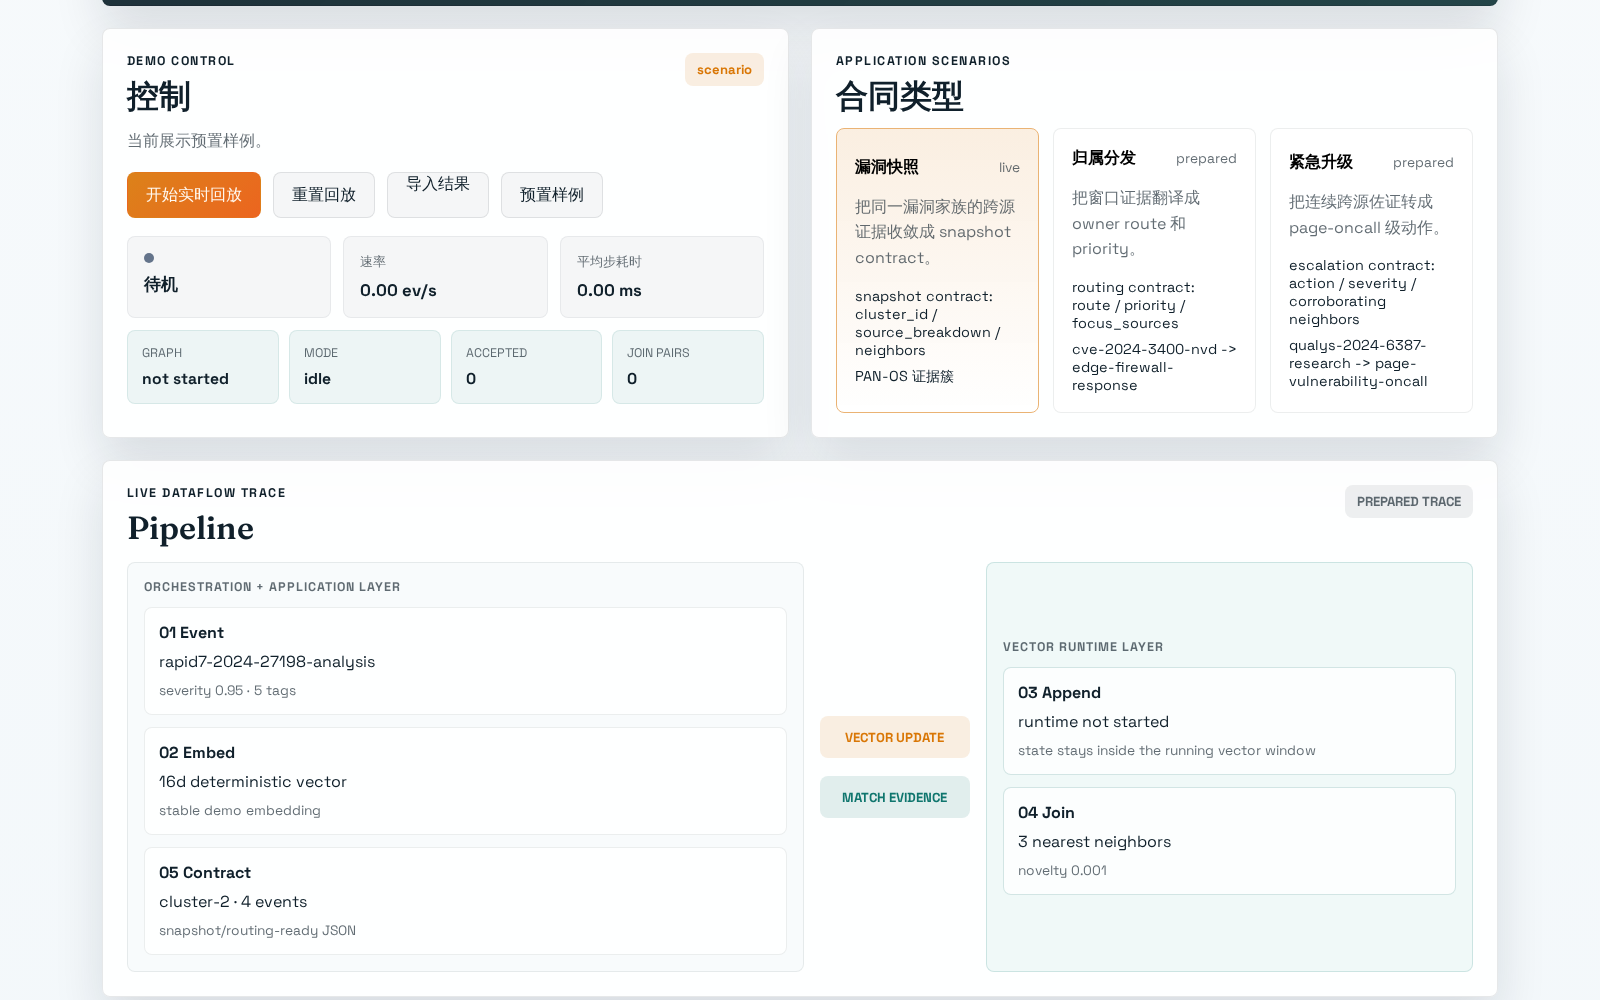
\includegraphics[width=0.82\textwidth,height=0.30\textheight,keepaspectratio]{figures/brisk_ui_walkthrough.png}
  \caption{Web interface for the demo. Controls, contract modes, runtime evidence, and prepared experiment summaries remain visible so the audience can connect UI actions with the semantic-window state underneath.}
  \Description{Screenshot of the BriskSnapShot web interface with replay controls, a pipeline trace, runtime metrics, active clusters, contracts, and experiment evidence.}
  \label{fig:ui}
\end{figure*}

\subsection{Audience Path}

Figure~\ref{fig:ui} shows the UI used in the demonstration. The left side controls the replay and displays the active pipeline trace. The right side shows contract scenarios and runtime evidence. The important UI choice is that the pipeline is not decorative: each row corresponds to a stage that changes system state. The event stage introduces a source report; the embedding stage makes the report comparable; the append stage changes the retained window; the join stage exposes which prior records matched; the contract stage shows what the application receives.

The presenter starts from an empty runtime and runs the stream one event at a time. Early events trigger emerging-risk contracts because the system has not yet seen enough related evidence. As reports from additional sources arrive, the same incident families become connected clusters and the UI switches from novelty to correlation. The audience can pause the replay, inspect the nearest neighbors supporting a cluster, and compare the current snapshot with the contract text that would be passed to a downstream service.

\begin{table}[t]
  \centering
  \caption{Presenter script for the live demo.}
  \label{tab:script}
  \begin{tabular}{@{}p{0.18\columnwidth}p{0.67\columnwidth}@{}}
    \toprule
    Step & What the audience sees \\
    \midrule
    Replay & Source, severity, timestamp, and embedding handoff for the current event \\
    Runtime & Retained records, emitted pairs, and nearest neighbors inside the active window \\
    Snapshot & Cluster membership, source coverage, novelty, and representative evidence \\
    Contract & Owner route, priority, recommended action, and supporting event identifiers \\
    Variant & How threshold, window size, or input order changes the visible contract stream \\
    \bottomrule
  \end{tabular}
\end{table}

Table~\ref{tab:script} is the actual demo script. The walkthrough is designed to answer five questions in order. What just arrived? What did the runtime retain? Which records joined? What compact evidence was exported? What changes when the audience asks for a different parameter setting? This is the same structure used in many systems demonstrations: start with a concrete user path, reveal internal state at the moment it matters, and close by showing robustness beyond the exact path shown on screen.

\subsection{Demonstration Scenarios}

The snapshot scenario shows why the bounded window matters. When the PAN-OS reports arrive from a vendor advisory, NVD, an emergency warning, and a research note, the system connects them into a single family and exports a compact summary with source coverage. The UI lets the audience see that the summary is not a generic LLM explanation; it is grounded in event identifiers and emitted join pairs.

The routing scenario shows how the same evidence can be converted into an owner decision. A VPN-related cluster is routed to the network perimeter owner because the source mix and severity cross the routing threshold. The presenter can open the route card, inspect the supporting neighbors, and show that route changes are tied to runtime evidence rather than keyword matching.

The escalation scenario focuses on high-severity novelty. A new report may not yet have enough neighbors for a dense cluster, but it can still become actionable if severity is high and novelty remains above threshold. This scenario is important for audience trust: the system is not only finding repeated topics; it also preserves a path for emerging risks that have not yet accumulated multiple sources.

\section{Prepared Evidence}
\label{sec:evidence}

The 24-event walkthrough is intentionally small enough for a live audience. To show more than a toy sample, the prepared evidence uses deterministic expanded replays. The expansion repeats the public-event templates with unique identifiers, shifted timestamps, and replay metadata. This keeps the semantics of the incident families understandable while increasing the number of events seen by the runtime.

\begin{figure}[t]
  \centering
  % Generated from data/prepared_demo_run.json and data/prepared_demo_evidence.json.
\resizebox{\columnwidth}{!}{%
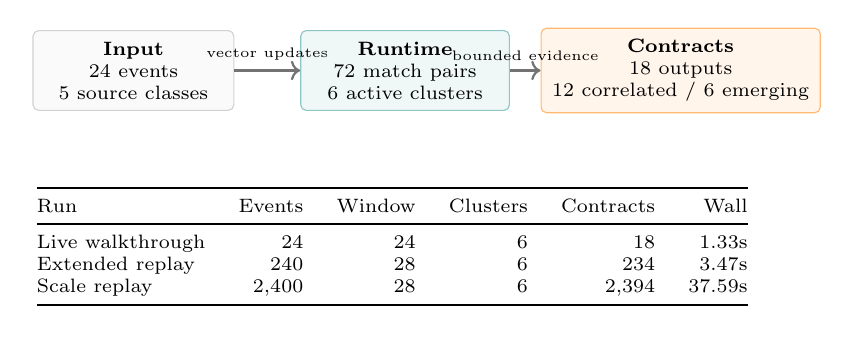
\begin{tikzpicture}[
  font=\scriptsize,
  box/.style={draw=black!18, rounded corners=2pt, fill=gray!4, inner sep=4pt, align=center},
  runbox/.style={draw=teal!45, rounded corners=2pt, fill=teal!6, inner sep=4pt, align=center},
  outbox/.style={draw=orange!55, rounded corners=2pt, fill=orange!8, inner sep=4pt, align=center},
  arrow/.style={->, thick, draw=black!55}
]
  \node[box, minimum width=2.55cm, minimum height=1.0cm] (input) at (0,2.8) {
    \textbf{Input}\\24 events\\5 source classes
  };
  \node[runbox, minimum width=2.65cm, minimum height=1.0cm] (runtime) at (3.45,2.8) {
    \textbf{Runtime}\\72 match pairs\\6 active clusters
  };
  \node[outbox, minimum width=2.75cm, minimum height=1.0cm] (contracts) at (6.95,2.8) {
    \textbf{Contracts}\\18 outputs\\12 correlated / 6 emerging
  };
  \draw[arrow] (input) -- node[above, font=\tiny] {vector updates} (runtime);
  \draw[arrow] (runtime) -- node[above, font=\tiny] {bounded evidence} (contracts);

  \node[anchor=north west, align=left] at (-1.35,1.45) {
    \begin{tabular}{@{}lrrrrr@{}}
      \toprule
      Run & Events & Window & Clusters & Contracts & Wall \\
      \midrule
    Live walkthrough & 24 & 24 & 6 & 18 & 1.33s \\
    Extended replay & 240 & 28 & 6 & 234 & 3.47s \\
    Scale replay & 2,400 & 28 & 6 & 2,394 & 37.59s \\
      \bottomrule
    \end{tabular}
  };
\end{tikzpicture}%
}

  \caption{Prepared result summary. The same demo path is run at three replay sizes; wall time is measured on the Python demo path and includes runtime startup.}
  \Description{A compact result figure showing input, runtime, and contract counts for the 24-event prepared run plus a scale table for 24, 240, and 2400 events.}
  \label{fig:results}
\end{figure}

\subsection{Workloads and Metrics}

The live workload has 24 events, five source classes, six incident families, and 18 exported contracts. The extended replay has 240 events and keeps a 28-record active window. The scale replay has 2,400 events with the same bounded window. We report four quantities because they map directly to the demo claims: active window size, number of active clusters, number of emitted contracts, and wall-clock time for the prepared Python demo path.

Figure~\ref{fig:results} shows the main result. The live run produces 72 match pairs, six active clusters, and 18 contracts. The 240-event replay produces 234 contracts in 3.47 seconds, while the 2,400-event replay produces 2,394 contracts in 37.59 seconds. The active window remains bounded at 28 records for the larger runs, so the final UI state remains inspectable even though the contract stream grows with the input.

\begin{table}[t]
  \centering
  \caption{Prepared parameter variants used during the demo.}
  \label{tab:variants}
  \begin{tabular}{@{}p{0.31\columnwidth}p{0.52\columnwidth}@{}}
    \toprule
    Variant & Expected visible effect \\
    \midrule
    Tighter threshold & Fewer join pairs, fragmented clusters, fewer correlated contracts \\
    Shorter window & Older incident families leave the snapshot earlier \\
    Reordered input & Same topic families, different contract reveal times \\
    Expanded replay & More emitted contracts while the final window stays bounded \\
    \bottomrule
  \end{tabular}
\end{table}

Table~\ref{tab:variants} lists the parameter variants that the presenter can switch to after the main walkthrough. These variants are included because a demo paper should not only describe the happy path. A tighter threshold tests whether the interface still explains why fewer clusters appear. A shorter window tests whether bounded retention is visible. Reordered input tests whether the system preserves incident families while changing the moment at which contracts become visible.

\subsection{What the Evidence Shows}

The prepared evidence supports three claims. First, the live path has enough data to show real behavior: the 24 reports produce multiple incident families, cross-source clusters, and both correlation and novelty contracts. Second, the runtime boundary remains usable as the input grows: the window is bounded, but contract emission continues. Third, the UI exposes the relevant system effect when parameters change. A demo attendee does not need to infer behavior from a hidden log; the state transition is visible through retained records, match pairs, clusters, and exported contracts.

\section{Discussion and Conclusion}

\system{} is a demonstration of a system boundary: semantic-window state remains inside a persistent vector runtime, while the application receives bounded contracts that are stable enough to inspect, log, route, and summarize. The key point is not that vector search can find similar records; the key point is that streaming vector evidence can become observable application behavior. The demo therefore emphasizes the handoff from event stream to runtime evidence to contract output.

There are two takeaways for attendees. The first is operational: a semantic window should expose enough state for a human to understand why an application-level decision changed. In \system{}, the presenter can point from a contract back to retained events and join pairs, which makes the system easier to debug than a pipeline that only displays generated text. The second takeaway is architectural: keeping the join state inside a long-lived runtime avoids rebuilding semantic context at every application step. This is what lets the demo show freshness, boundedness, and contract emission as one continuous behavior.

The demo also makes its current limitations visible. The replay uses deterministic embeddings so that the audience can reproduce the same sequence of clusters and contracts; a deployed system would replace that stage with a production embedding service and would need monitoring for embedding drift. The contract rules are intentionally simple threshold rules, which makes the UI explainable but leaves room for learned policies or organization-specific routing constraints. These limitations are useful in a demonstration setting because they separate the systems contribution from policy choices that can vary across applications.

The current prototype focuses on vulnerability intelligence because the domain makes semantic grouping and escalation easy to understand. The same pattern applies to other streaming AI tasks where new evidence must be incorporated during a long-running workflow: customer-support incidents, scientific-monitoring feeds, or operational telemetry. Future extensions will make the contract rules learned or policy-driven, but the live demo already exposes the essential systems question: how can an AI pipeline keep semantic context fresh without hiding the runtime state that justifies its actions?

\bibliographystyle{ACM-Reference-Format}
\bibliography{References}

\end{document}
